In this section, we apply the adaptive correlation thresholding method to a portfolio construction problem. First we describe the procedure and then present some of the results we have. 

Assume we observe the excess return \(Y_{it}\), \(i = 1,\dots,N\) and \(t= 1,\dots, T\) follows
\begin{equation*}
    Y_{it} = B_{i}' F_{t} + u_{it} ; \quad \Sigma_{u} = E(u_{t}u_{t}')
\end{equation*}
where \(F_{t}\) are factor excess returns. Here we have considered Fama-French 3 and the Carhart's momentum factor. The goal is to estimate \(\Sigma_{Y} = E\pqty{YY'}\) and use that estimate to construct portfolio following \cite{ledoit2017NonlinearShrinkage}. The auxialiary network we have include the \cite{hoberg2016TextBasedNetwork}'s network(henceforth Hoberg's Network) and IBES analysts cocoverage network. Here we present the results for SP500 returns using Hoberg's Network. 

The procedure we take is as follows. 
\begin{enumerate}
    \item We run time series linear regressions of \(Y_{it}\) on \(F_{k,t}\), obtain the beta estimates \(\hat{B}_{i}\) and the residual \(\hat{u}_{it}\). 
    \item Compute the covaraince matrix \(S_{\hat{u}} = \frac{1}{T}\hat{u}\hat{u}'\) and \(S_{F} = \frac{1}{T} \sum_{t} (F_{t} - \bar{F})(F_{t} - \bar{F})'\) and appply \textit{adaptive correlation thresholding} on \(S_{\hat{u}}\), denote the estimate as \(\hat{S}_{\hat{u}}\). 
where the second step adaptive correlation thresholding is achieved in the following way. Let \(R_{u}\) be the correlation matrix calculated from \(S_{u}\). We use soft thresholding \(h(r_{ij}, \tau_{ij}) = \sign\pqty{r_{ij}} \pqty{r_{ij} - \tau_{ij}}_{+}\) on the off-diagonal elemetns \(r_{ij}\) of \(R_{u}\), where 
\begin{equation*}
    \tau_{ij} = \delta_{ij} \sqrt{\frac{\log N}{T}}
\end{equation*}
and 
\begin{equation*}
    \delta_{ij} = a + b G_{ij}
\end{equation*}

% \blue{(so that the network is a little denser, and I have also considered specification of \(\delta\) as a probit model, but it complicates the optimization part because the constraint is nonlinear.)}. 

Let the threshold estimate be \(\hat{R}_{\hat{u}}(a,b)\), given \(a,b\), our estimate will be
\begin{equation*}
    \hat{S}_{\hat{u}} = \hat{S}_{\hat{u}}(a,b) = \diag(S_{\hat{u}})^{\frac{1}{2}} \hat{R}_{\hat{u}}\diag(S_{\hat{u}})^{\frac{1}{2}}
\end{equation*}

In order to guarantee positive definiteness, I follow the suggestion in \cite{fan2015OverviewEstimation} and \cite{fan2013LargeCovariance}, by first finding the minimum \(\underline{\delta}\) such that the \(\hat{S}(\delta, 0)\) has its smallest eigenvalue larger than \(0\) if we choose \(\tau_{ij} = \underline{\delta} \sqrt{\frac{\log N}{T}}\). 

Then \(a,b\) are estimated using cross-validation following \cite{bickel2008CovarianceRegularization} by randomly spliting the sample \(V\) times, for each \(v = 1,\dots,V\), compute the estimate \(\hat{S}^{1,v}_{u}\) with the first subsample, and sample covariance estimate \(\hat{\Sigma}^{2,v}_{u}\) with the second subsample and let the criterion function be
\begin{equation*}
    L(a, b) = \frac{1}{V} \sum_{v}^{V} \norm{\hat{S}^{1,v}_{u} - \hat{\Sigma}^{2,v}_{u}}^{2}_{F}
\end{equation*}
we find \(\hat{a},\hat{b}\) that minimise this criterion subject to the constraints:
\begin{align}
    0 \leq a \sqrt{\frac{\log N}{T}} &\leq 1 \\
    b \sqrt{\frac{\log N}{T}} &\leq 0 \\
    \underline{\delta} &\leq a + b 
\end{align}
\item Construct an estimate of \(\Sigma_{Y}\) by \(\hat{\Sigma}_{Y} = \hat{B}S_{F}\hat{B}' +\hat{S}_{\hat{u}}\)
\end{enumerate}

We have estimated the covariance matrices of SP500 stocks from 1996 to the end of 2017; using stock return data and Fama-French 3 factor returns \(F_{kt}, k =1,2,3\). We incorporate Hoberg's network \(G_{t}\) that are updated yearly into our estimation procedure. 

The Hoberg's Network is a yearly updated \(N\times N\) network with elements in \([0,1]\) with higher score \(G_{ij}\) reflecting potentially higher correlation between the \(i\)-th and \(j\)-th firms.


In Figure 1, we present the distribution, we present the distribution (blue) of sample covariance estimates \(S_{\hat{u}, ij}\) of residuals after regressing the the stocks returns on the Fama-French 3 factor for the stocks that haIn Figure 1, we present the distribution (blue) of sample covariance estimates \(S_{\hat{u}, ij}\) of residuals after regressing the the stocks returns on the Fama-French 3 factor for the stocks tsiduals after regressing the the stocks returns on the Fama-French 3 factor for the stocks that have no missing data in the dataset; alongwith the distribution of  sample covariance \(S_{\hat{u},ij}\) for those \(ij\) with \(G_{ij} > 0\) in the Hoberg's network. It's clear that the distribution is shifted to the right, implying that Hoberg's network can pick up information that are not explained by the factors. 

\begin{figure}[htbp]
    \centering
    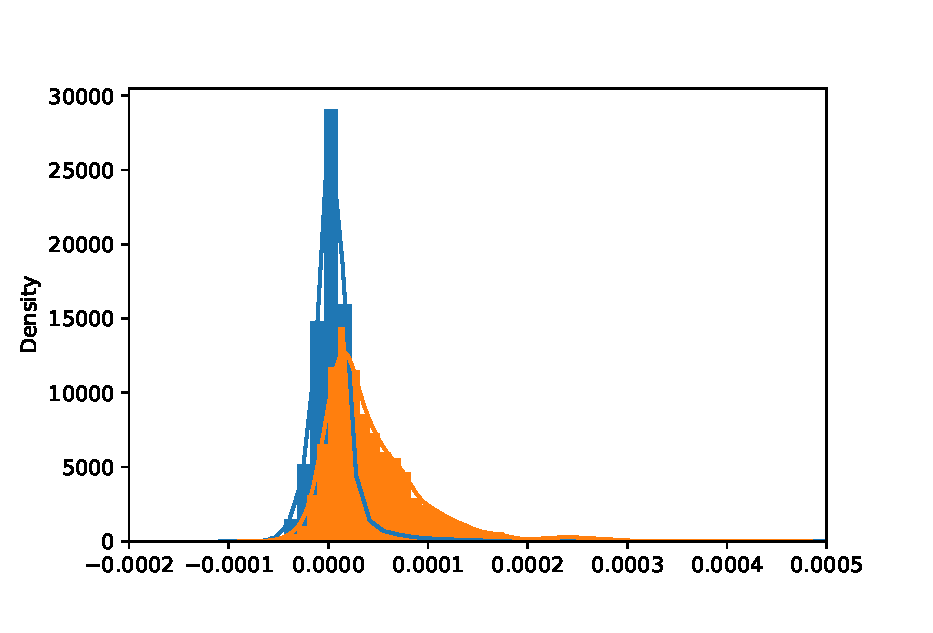
\includegraphics{fig1.eps}
    \caption{Distribution of \(S_{\hat{u},ij}, i,j = 1,\dots,N\) and \(S_{\hat{u},ij}\) for \(i,j\) such that \(G_{ij} >0\) }
    \label{<label>}
\end{figure}

Then we use a rolling-window estimation, with 252-day estimation period and then move the window forward by 21 days. In the estimation periods in window  \(m= 1, \dots,M\) we construct estimate \(\hat{\Sigma}_{Y,m} = \hat{B}S_{F}\hat{B}' + \hat{S}_{\hat{u}}\pqty{\hat{a}_{m}, \hat{b}_{m}}\). The estimated parameters \(\hat{a}_{m},\hat{b}_{m} \)  have mean \((1.177, -0.252)\), where the \(\hat{b}\) measures the effect of knowing the auxiliary network on the thresholding level. 
